\documentclass[10pt,english]{article}
\usepackage[T1]{fontenc}
\usepackage[latin9]{inputenc}
\usepackage{geometry}
\geometry{verbose,tmargin=1.5in,bmargin=1.5in,lmargin=1.5in,rmargin=1.5in}
\usepackage{amsthm}
\usepackage{amsmath}
\usepackage{amssymb}
\usepackage{pgfplots}

\makeatletter
\usepackage{enumitem}
\newlength{\lyxlabelwidth}

\usepackage[T1]{fontenc}
\usepackage{ae,aecompl}

%\usepackage{txfonts}

\usepackage{microtype}

\usepackage{calc}
\usepackage{enumitem}
\setenumerate{leftmargin=!,labelindent=0pt,itemindent=0em,labelwidth=\widthof{\ref{last-item}}}

\makeatother

\usepackage{babel}
\begin{document}
\noindent \begin{center}
\textbf{\large{}MATH 146 - Assignment 1}\\
\textbf{\large{}Chris Ji 20725415}
\par\end{center}{\large \par}
\medskip{}

\begin{enumerate}
\item \begin{enumerate}
    \item A corresponding symmetric matrix for $Q(x_1,x_2)$ is $A=\begin{bmatrix}5&-2\\-2&2\end{bmatrix}$. We see that $\text{det}\left(\begin{bmatrix}5-\lambda&-2\\-2&2-\lambda\end{bmatrix}\right)=\lambda^2-7\lambda+6=(\lambda-1)(\lambda-6)$. Hence all of the eigenvalues are positive, and $Q(\vec{x})$ and $A$ are positive definite. By theorem 10.3.1 there exists an orthogonal matrix $P$ such that $\vec{y}=P^T\vec{x}$ gives $Q(\vec{x})=y_1^2+6y_2^2$. \\ 
    For $\lambda_1=1$, $A-\lambda_1I\sim\begin{bmatrix}1&-\frac{1}{2}\\0&0\end{bmatrix}$, so an orthonormal basis for this eigenspace is $\left\{\begin{bmatrix}\frac{1}{\sqrt{5}}\\\frac{2}{\sqrt{5}}\end{bmatrix}\right\}$. \\ 
    For $\lambda_2=6$, $A-\lambda_2I\sim\begin{bmatrix}1&2\\0&0\end{bmatrix}$, so an orthonormal basis for this eigenspace is $\left\{\begin{bmatrix}\frac{-2}{\sqrt{5}}\\\frac{1}{\sqrt{5}}\end{bmatrix}\right\}$. \\ 
    Then $P=\begin{bmatrix}\frac{1}{\sqrt{5}}&\frac{-2}{\sqrt{5}}\\\frac{2}{\sqrt{5}}&\frac{1}{\sqrt{5}}\end{bmatrix}$, and $P^TAP=\begin{bmatrix}1&0\\0&6\end{bmatrix}$, as expected, and the change of variables $\vec{y}=\begin{bmatrix}\frac{1}{\sqrt{5}}&\frac{2}{\sqrt{5}}\\\frac{-2}{\sqrt{5}}&\frac{1}{\sqrt{5}}\end{bmatrix}\vec{x}$ gives us $Q(\vec{x})=y_1^2+6y_2^2$.
    \pagebreak
    \item A corresponding symmetric matrix for $Q(x_1,x_2,x_3)$ is $A=\begin{bmatrix}1&-1&3\\-1&1&3\\3&3&-3\end{bmatrix}$. We see that $\text{det}\left(\begin{bmatrix}1-\lambda&-1&3\\-1&1-\lambda&3\\3&3&-3-\lambda\end{bmatrix}\right)=-\lambda^3-\lambda^2+24\lambda-36=-(\lambda-2)(\lambda-3)(\lambda+6)$. Since two eigenvalues are positive, and one is negative, $Q(\vec{x})$ and $A$ are indefinite. Note that by theorem 10.3.1 there exists an orthogonal matrix $P$ such that $\vec{y}=P^T\vec{x}$ gives $Q(\vec{x})=2y_1^2+3y_2^2-6y_3^2$\\ 
    For $\lambda_1=2$, $A-\lambda_1I\sim\begin{bmatrix}1&1&0\\0&0&1\\0&0&0\end{bmatrix}$, so an orthonormal basis for this eigenspace is $\left\{\begin{bmatrix}-\frac{1}{\sqrt{2}}\\\frac{1}{\sqrt{2}}\\0\end{bmatrix}\right\}$. \\ 
    For $\lambda_2=3$, $A-\lambda_2I\sim\begin{bmatrix}1&0&-1\\0&1&-1\\0&0&0\end{bmatrix}$, so an orthonormal basis for this eigenspace is $\left\{\begin{bmatrix}\frac{1}{\sqrt{3}}\\\frac{1}{\sqrt{3}}\\\frac{1}{\sqrt{3}}\end{bmatrix}\right\}$.\\ 
    For $\lambda_3=-6$, $A-\lambda_3I\sim\begin{bmatrix}1&0&\frac{1}{2}\\0&1&\frac{1}{2}\\0&0&0\end{bmatrix}$, so an orthonormal basis for this eigenspace is $\left\{\begin{bmatrix}-\frac{1}{\sqrt{6}}\\-\frac{1}{\sqrt{6}}\\\sqrt{\frac{2}{3}}\end{bmatrix}\right\}$.\\ 
    Then $P=\begin{bmatrix}-\frac{1}{\sqrt{2}}&\frac{1}{\sqrt{3}}&-\frac{1}{\sqrt{6}}\\\frac{1}{\sqrt{2}}&\frac{1}{\sqrt{3}}&-\frac{1}{\sqrt{6}}\\0&\frac{1}{\sqrt{3}}&\sqrt{\frac{2}{3}}\end{bmatrix}$, and $P^TAP=\begin{bmatrix}2&0&0\\0&3&0\\0&0&-6\end{bmatrix}$, as expected, and the change of variables $\vec{y}=\begin{bmatrix}-\frac{1}{\sqrt{2}}&\frac{1}{\sqrt{2}}&0\\\frac{1}{\sqrt{3}}&\frac{1}{\sqrt{3}}&\frac{1}{\sqrt{3}}\\-\frac{1}{\sqrt{6}}&-\frac{1}{\sqrt{6}}&\sqrt{\frac{2}{3}}\end{bmatrix}\vec{x}$ gives us $Q(\vec{x})=2y_1^2+3y_2^2-6y_3^2$.
\end{enumerate}

\pagebreak
\item Note that a symmetric matrix for this equation is $\begin{bmatrix}3&2\\2&3\end{bmatrix}$, and $\text{det}\left(\begin{bmatrix}3-\lambda&2&\\2&3-\lambda\end{bmatrix}\right)=\lambda^2-6\lambda+5=(\lambda-1)(\lambda-5)$. Then the change of variables $\vec{y}=P^T\vec{x}$ gives us $5=y_1^2+5y_2^2$, which gives us an ellipse with center (0,0), and setting $y_1$ as the x axis, intersects the axes at $(\sqrt{5},0),(\sqrt{5},0),(0,1),(0,-1)$. By theorem 10.4.1, we know the graph of $3x_1^2+4x_1x_2+3x_2^2=5$ will be a rotation of this one. To change the graph from the $y_1y_2-$plane to the $x_1x_2-$plane, we find $P$. The unit eigenvector for $\lambda_1=1$ is $\begin{bmatrix}-\frac{1}{\sqrt{2}}\\\frac{1}{\sqrt{2}}\end{bmatrix}$, and the unit vector for $\lambda_2=5$ is $\begin{bmatrix}\frac{1}{\sqrt{2}}\\\frac{1}{\sqrt{2}}\end{bmatrix}$, so $P=\begin{bmatrix}-\frac{1}{\sqrt{2}}&\frac{1}{\sqrt{2}}\\\frac{1}{\sqrt{2}}&\frac{1}{\sqrt{2}}\end{bmatrix}$. Notice that the $y_1$ axis is just the line spanned by $\begin{bmatrix}1\\0\end{bmatrix}$. Then $\vec{x}=[\vec{v}_1\quad\vec{v}_2]\begin{bmatrix}1\\0\end{bmatrix}=\vec{v}_1$, and so the $y_1-$axis in the $x_1x_2-$plane is the line spanned by $\vec{v}_1$. Similarly $y_2$ is spanned by $\begin{bmatrix}0\\1\end{bmatrix}$, and so the $y_2-$axis in the $x_1x_2-$plane is the line spanned by $\vec{v}_2$. 


\pagebreak
\leavevmode\vadjust{\vspace{-\baselineskip}}\newline
\begin{tikzpicture}
\begin{axis}[axis lines = middle, xmin=-2.25, xmax=2.25, ymin=-1, ymax=1,xlabel = $y_1$,ylabel = {$y_2$}] 
\addplot [domain=-5:5, samples=5000, color=black]{sqrt{(5-x^2)/5}};
\addplot [domain=-5:5, samples=5000, color=black]{-sqrt{(5-x^2)/5}};
\end{axis}\end{tikzpicture}
Figure 1


\leavevmode\vadjust{\vspace{-\baselineskip}}\newline
%THIS IS THE ROTATED THING INSERTED INTO THE OTHER GRAPH
\newsavebox\insertedgraph
\savebox\insertedgraph
 {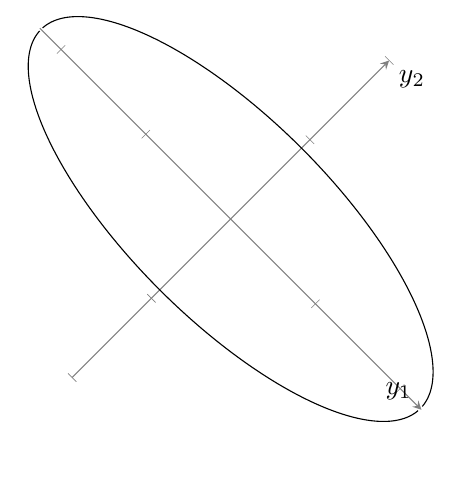
\begin{tikzpicture}
\begin{axis}[anchor=origin, rotate around={-45:(current axis.origin)}, axis lines = middle,
    xmin=-2.25, xmax=2.25, ymin=-1, ymax=1, xlabel = $y_1$, ylabel = {$y_2$},yticklabels=\empty,xticklabels=\empty,axis line style = gray] 
\addplot [domain=-5:5, samples=5000, color=black]{sqrt{(5-x^2)/5}};
\addplot [domain=-5:5, samples=5000, color=black]{-sqrt{(5-x^2)/5}};
\end{axis} \end{tikzpicture}}
  
\begin{tikzpicture}
  \begin{axis}
  [axis lines = middle, xmin=-2.25, xmax=2.25, ymin=-1, ymax=1,xlabel = $x_1$,ylabel = {$x_2$}] 
  %FOLLOWING 2 LINES INSERTS THE GRAPH
  \node at (axis cs: 0,0)
    {\scalebox{1}{\usebox\insertedgraph}};
  \end{axis}
\end{tikzpicture}
Figure 2

\pagebreak
\item $\langle\vec{x},\vec{x}\rangle=\frac{1}{2}[Q(\vec{x}+\vec{x})-Q(\vec{x})-Q(\vec{x})]=\frac{1}{2}Q(2\vec{x})$. Note that since $Q(\vec{x})$ is positive definite, $\frac{1}{2}Q(2\vec{x})>0$ for all $\vec{x}\neq0$, and $\frac{1}{2}Q(2\vec{0})=0$, so $\langle\vec{x},\vec{x}\rangle=0$ for $\vec{x}=\vec{0}$. So $\langle\vec{x},\vec{y}\rangle$ is positive definite.\\ 
$\langle\vec{x},\vec{y}\rangle=\frac{1}{2}[Q(\vec{x}+\vec{y})-Q(\vec{x})-Q(\vec{y})]=\frac{1}{2}[Q(\vec{y}+\vec{x})-Q(\vec{y})-Q(\vec{x})]=\langle\vec{y},\vec{x}\rangle$, so $\langle\vec{x},\vec{y}\rangle$ is symmetric. \\ 
Let $A$ be the corresponding matrix to $Q(\vec{x})$. Then 
\begin{align*}\langle a\vec{x}+b\vec{y},\vec{z}\rangle&=\frac{1}{2}[Q(a\vec{x}+b\vec{y}+\vec{z})-Q(a\vec{x}+b\vec{y})-Q(\vec{z})]\\&=(a\vec{x}+b\vec{y}+\vec{z})^TA(a\vec{x}+b\vec{y}+\vec{z})-(a\vec{x}+b\vec{y})^TA(a\vec{x}+b\vec{y})-\vec{z}^TA\vec{z}\\&=(a\vec{x}^TAa\vec{x}+b\vec{y}^TA\vec{y}+\vec{z}^TA\vec{z})-(a\vec{x}^TA\vec{x}+b\vec{y}^TA\vec{y})-(\vec{z}^TA\vec{z})=\vec{0}
\end{align*} Note that 
\begin{align*}a\langle\vec{x},\vec{z}\rangle+b\langle\vec{y},\vec{z}\rangle&=a\frac{1}{2}[Q(\vec{x}+\vec{z})-Q(\vec{x})-Q(\vec{z})]+b\frac{1}{2}[Q(\vec{y}+\vec{z})-Q(\vec{y})-Q(\vec{z})]\\&=a\frac{1}{2}[\vec{x}^TA\vec{x}+\vec{z}^TA\vec{z}-\vec{x}^TA\vec{x}-\vec{z}^TA\vec{z}]+b\frac{1}{2}[\vec{y}^TA\vec{y}+\vec{z}^TA\vec{z}-\vec{y}^TA\vec{y}-\vec{z}^TA\vec{z}]=\vec{0}\end{align*}
So $\langle\vec{x},\vec{y}\rangle$ is bilinear.\\ 
Since $\langle\vec{x},\vec{y}\rangle$ is positive definite, symmetric, and bilinear, it is an inner product on $\mathbb{R}^n$. 

\pagebreak
\item \begin{enumerate}
    \item If $A$ is a positive definite symmetric matrix, then it does not have an eigenvalue of 0 (as they are all strictly positive). Then by invertible matrix theorem, $A$ is invertible. (This is not in our MATH136 invertible matrix theorem, so I provided a proof below) \\\\
    \textbf{Theorem: a matrix $A$ is not invertible if $0$ is an eigenvalue of $A$}\\ 
    Assume $A$ is an invertible matrix with $0$ as an eigenvalue. Then $(A-\lambda I)\cdot\vec{v}=\vec{0}$ with $\lambda=0$. But then if $\lambda=0$, $(A-\lambda I)=A\Rightarrow A\vec{v}=\vec{0}$. Then by the fact that $A$ is invertible, $\vec{v}$ must be $\vec{0}$. But the zero vector cannot be an eigenvector, so $0$ cannot be an eigenvalue of an invertible matrix. 
    
    %GIVE KRISTI INDUCTION
    
    \item Note that for any $\vec{x}$ corresponding to a (positive eigenvalue) $\lambda$, $A\vec{x}=\lambda\vec{x}$. \begin{align*}A\vec{x}&=\lambda\vec{x}\\A^{-1}A\vec{x}&=A^{-1}\lambda\vec{x}\\\vec{x}=\lambda A^{-1}\vec{x}\\\frac{1}{\lambda}\vec{x}=A^{-1}\vec{x}\end{align*} So $\frac{1}{\lambda}$ is an eigenvalue of $A^{-1}$. Note that all $\lambda$'s of $A$ are positive, so $\frac{1}{\lambda}$ must be positive for any $\lambda$, and so $A^{-1}$ is positive definite. 
    
    \item Let $P^TAP=B$, for some matrix $B$. Then by question 5c on the last assignment, $B$ is orthogonally diagonalizable (as it is orthogonally similar to a symmetric matrix). Then for some orthogonal matrix $Q$, $Q^TBQ=D$, for some diagonal matrix $D$ (note that $D$'s diagonal is the eigenvalues of $B$, which we want to show are all positive for $P^TAP$ to be positive definite). Then $Q^TP^TAPQ=D$. Note that $Q^TP^T$ and $PQ$ are both orthogonal matrices, so $A$ is orthogonally diagonalizable by orthogonal matrix $PQ$, into a diagonal matrix $D$. But we know $A$ and $D$ must share eigenvalues, and all of $A$'s eigenvalues are positive. $D$ also shares eigenvalues with $B$, and so all of $B$'s eigenvalues are positive, and so $B$ is positive definite. 
\end{enumerate}

\pagebreak
\item Taking the hint, suppose $Q$ diagonalizes $A$ to $D$, so that $Q^TAQ=D$. Define a matrix $C$ such that $C^2=D$, and let $B=QCQ^T$. Then we see that $Q^TAQ=C^2\Rightarrow A=QC^2Q^T$. Note that $B=QCQ^T\Rightarrow BB=QCQ^TQCQ^T\Rightarrow B^2=QCCQ^T\Rightarrow B^2=QC^2Q^T$ (since $Q^T=Q{-1}$, $Q^TQ=I$). Then $A=QC^2Q^T=B^2$, as required. 


\end{enumerate}

\end{document}
